\providecommand{\pgfsyspdfmark}[3]{}
\providecommand{\savepicturepage}[3]{}

\documentclass[11pt,letterpaper]{article}
\usepackage[lmargin=1in,rmargin=1in,tmargin=1in,bmargin=1in]{geometry}

% -------------------
% Packages
% -------------------
\usepackage{
	amsmath,			% Math Environments
	amssymb,			% Extended Symbols
	enumerate,		    % Enumerate Environments
	graphicx,			% Include Images
	lastpage,			% Reference Lastpage
	multicol,			% Use Multi-columns
	multirow,			% Use Multi-rows
	gensymb
}


% -------------------
% Font
% -------------------
\usepackage[T1]{fontenc}
\usepackage{charter}
\usepackage{xcolor}

% -------------------
% Commands
% -------------------

\newcommand{\prob}{\noindent\textbf{Problem. }}
\newcounter{problem}
\newcommand{\problem}{
	\stepcounter{problem}%
	\noindent \textbf{Problem \theproblem. }%
}
\newcommand{\answer}{\noindent \textbf{Answer. }}
\newcommand{\pspace}{\par\vspace{\baselineskip}}
\newcommand{\ds}{\displaystyle}


% -------------------
% Header & Footer
% -------------------
\usepackage{fancyhdr}

\fancypagestyle{pages}{
	%Headers
	\fancyhead[L]{}
	\fancyhead[C]{}
	\fancyhead[R]{}
\renewcommand{\headrulewidth}{0pt}
	%Footers
	\fancyfoot[L]{}
	\fancyfoot[C]{}
	\fancyfoot[R]{}
\renewcommand{\footrulewidth}{0.0pt}
}
\headheight=0pt
\footskip=14pt

\pagestyle{pages}


% -------------------
% Content
% -------------------
\begin{document}
\noindent\textbf{\large Calculus I (AM\_\_1050AH / MSF\_10110) \\ 2022 Fall \\ Differentiation rules III, IV}

\bigskip

\problem Find the following limits. You \textit{may} use L'Hôpital's rule \textit{if applicable}.
\begin{enumerate}[(a)]
    \item $\lim\limits_{x \to 1} \frac{\ln x}{\ln(x^3 + e^x)}$
    \item $\lim\limits_{x \to (-2)} \frac{\sin(\pi x)}{x^2-4}$
    \item $\lim\limits_{x \to \infty} \frac{x^2 + e^{4x}}{2x-e^x}$
    \item $\lim\limits_{x \to \infty} \frac{e^x-e^{-x}}{e^x+e^{-x}}$
    \item $\lim\limits_{x \to \infty} \sqrt[x]{x}$   (Hint: Show this is a $\infty^0$ form. Try evaluating the limit of its logarithm)
\end{enumerate}\vspace{6mm}

\noindent\begin{minipage}{0.7\textwidth}
    \problem Suppose we have $x^2+y^3=4$,
    \begin{enumerate}[(a)]
        \item Express $y$ as terms of $x$.
        \item Find $\frac{dy}{dx}$ using the expression in (a).
        \item Find $\frac{dy}{dx}$ using implicit differentiation on $x^2+y^3=4$.
        \item Show that the results in (b) and (c) are identical.
    \end{enumerate}
\end{minipage}
\begin{minipage}{0.3\textwidth}
    \begin{center}
        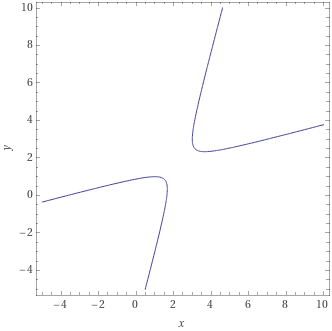
\includegraphics[width = \textwidth]{../graph/A09.png}
    \end{center}
\end{minipage}
\vspace{6mm}


\problem A hyperbola $\Gamma$ on a Cartesian plane can be described as $\Gamma:x^2-4xy+y^2+2x+6y-6=0$, which is graphed above:
\begin{enumerate}[(a)]
    \item Find all points on $\Gamma$ that has $x$-coordinate of 1.
    \item Find the tangent line(s) of $\Gamma$ at the point(s) in (a).
    \item Find all tangent lines of $\Gamma$ that are horizontal.
    \item Find all tangent lines of $\Gamma$ that are vertical. (Hint: At where tangent lines are vertical, $\frac{dx}{dy} = 0$)
\end{enumerate}\vspace{6mm}


\problem Evaluate the following high-order derivatives
\begin{enumerate}[(a)]
    \item $\frac{d^2}{dx^2}(e^{-x}\sin x)$
    \item $\frac{d^2}{dx^2}\ln(\ln x)$
    \item $\frac{d^6}{dx^6}(x^5 + 7x^4 + 3x^3 + 2x + 1)$
    \item $\frac{d^{10}}{dx^{10}} e^x$
    \item $\frac{d^{10}}{dx^{10}}\cos 2x$
\end{enumerate}\vspace{6mm}

% \problem Use the hinted linear approximations to approximate the following quantities:
% \begin{enumerate}[(a)]
%     \item $\tan 46 \degree$, approximating $\tan x$ at $x = 45 \degree$. (Note: You'll have to operate in radians) 
%     \item $\ln(1.01)$, approximating $\ln (1+x)$ at $x = 0$.
%     \item $\tan^{-1}0.99$, approximating $\tan^{-1} x$ at $x = 1$.
%     \item $\sqrt[4]{80}$, approximating $3\sqrt[4]{1+x}$ at $x = 0$.
%     \item $\frac{1}{0.99^3}$, approximating $\frac{1}{(1+x)^3}$ at $x = 0$.
% \end{enumerate}\vspace{6mm}

% \problem Find the following limits. You \textit{may} use the L'Hôpital's rule \textit{if applicable}.
% \begin{enumerate}[(a)]
%     \item $\lim\limits_{x \to 1} \frac{x^3+x^2+x-3}{x^3+2x^2+x-3}$
%     \item $\lim\limits_{x \to 0} \frac{e^{(3x^2+2x)}-1}{\sin(2x^2+3x)}$
%     \item $\lim\limits_{x \to 0} \frac{\sin (x^2)}{x \tan x}$
%     \item $\lim\limits_{x \to 0} x^2 \ln (x^2)$ \quad (Hint: Transform it into $\frac{\infty}{\infty}$ form)
%     \item $\lim\limits_{x \to 0} \frac{e^{-\frac{1}{x^2}}}{x^2}$ \quad (Hint: $\frac{0}{0}$ form can also be transformed into $\frac{\infty}{\infty}$ form)
% \end{enumerate}\vspace{4mm}

% \problem Determine if the following statements are true or false and explain. (You can just provide a counterexample if you determine them as false)
% \begin{enumerate}[(a)]
%     \item If $f'(x) = g'(x)$ (for all $x\in \mathbb{R}$), then $f(x) = g(x)$
%     \item If $f(1) = 0$, then $f'(1) = 0$
%     \item If $f'(x) = 0$ (for all $x\in \mathbb{R}$), then $f(x) = 0$
% \end{enumerate}\vspace{6mm}

% \problem Let $f(x) = \sqrt[4]{x} - \sqrt{x}$,
% \begin{enumerate}[(a)]
%     \item Find the tangent line of $f(x)$ at the point where $x=16$.
%     \item At which point(s) on $f(x)$ is its tangent line horizontal?
%     \item Is $f(x)$ differentiable at $x = 0$? Why?
% \end{enumerate}\vspace{6mm}

% \problem A ball is expanding with its radius $r$ as a function of time $t$: $r(t) = \sqrt{t} + 2, t \ge 0$
% \begin{enumerate}[(a)]
%     \item Find the rate its radius is growing at $t = 1$
%     \item Find the rate its surface area is growing at $t = 1$
%     \item Find the rate its volume is growing at $t = 1$
% \end{enumerate}\vspace{6mm}

\end{document}